\section{\textsc{Raw vegetable salad with apple}}

\subsection*{Ingredients for 2 portions:}

\begin{tabular}{p{7.5cm} p{7.5cm}}
	& \\
	\sfrac{1}{2} white cabbage & 3tbsp olive oil \\
	2 carrots & 3tbsp white vine vinegar \\
	1 apple & 1tbsp salt \\
	\multicolumn{2}{l}{papper, sugar, caraway to taste}
\end{tabular}

\subsection*{Serving suggestion:}

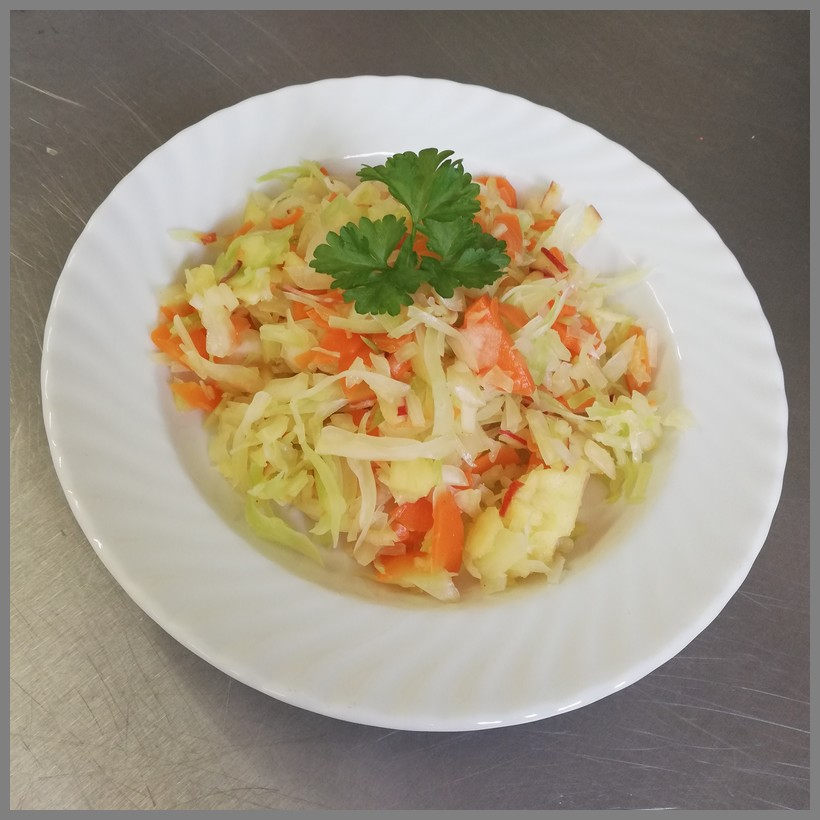
\includegraphics[width=\textwidth]{img/krautsalat_apfel.jpg} \cite{rohkostapfel}

\subsection*{How it's done:}

\begin{tabular}{p{15cm}}
	\\
  Peel and finely plane the carrots and apples.\\
  Cut the white cabbage into narrow strips with a large knife.\\
  Place the white cabbage in a large bowl and season with salt.\\
  Knead the cabbage until it forms its own juice. Add apples and carrots.\\
  Mix oil and vinegar. Season and season to taste.\\
  Pour over the vegetable mix and stir well.\\
  Allow to stand for at least 1-2 hours.
\end{tabular}
